\documentclass{article}
\usepackage{Sweave}
\begin{document}
\input{rsweave1-concordance}

% This is a comment
 
\begin{Schunk}
\begin{Sinput}
> # help("RweaveLatex")
> # this is an R code chunk.  R code goes in here, 
> # between the angle brackets and the at symbol.
> a = 123456
> print(a)
\end{Sinput}
\begin{Soutput}
[1] 123456
\end{Soutput}
\end{Schunk}


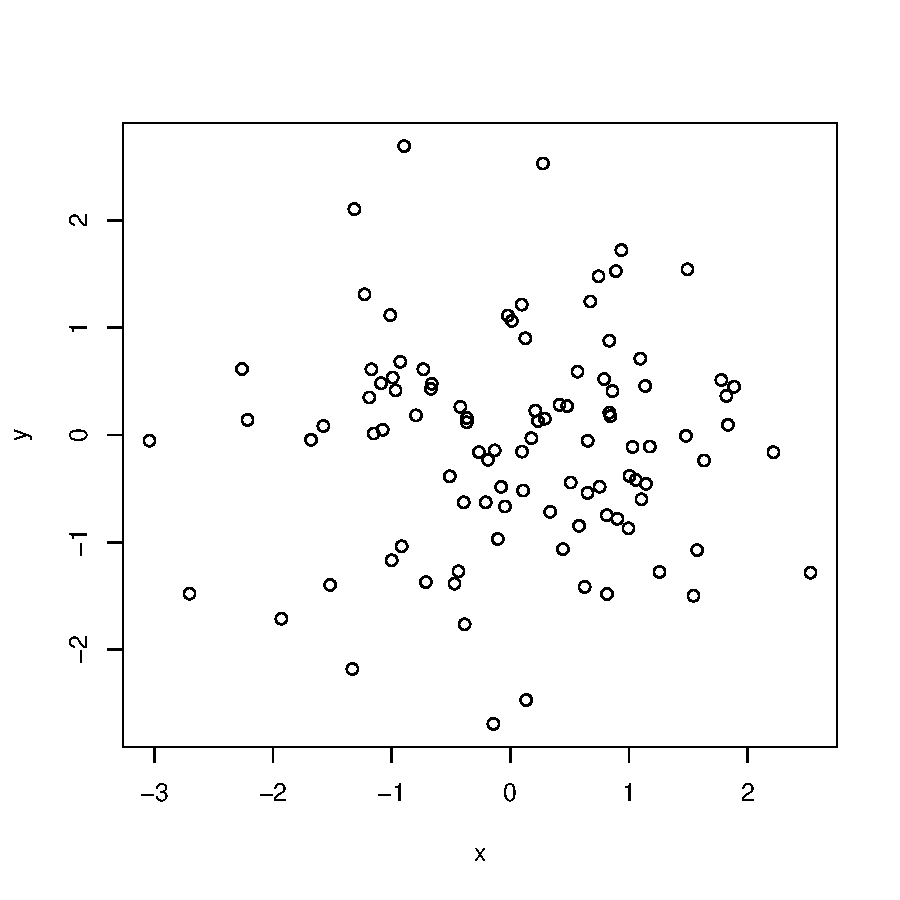
\includegraphics{rsweave1-003}

\begin{Schunk}
\begin{Soutput}
    a.b.c.d 
 3 4 3 5:1  
\end{Soutput}
\end{Schunk}
\end{document}

